\documentclass{article}

\usepackage[utf8]{inputenc}
\usepackage[T1]{fontenc}
\usepackage{lipsum}
\usepackage{graphicx}
\usepackage{amsmath}
\usepackage[margin=1in]{geometry}
\usepackage{titlesec}

\titleformat{\section}
{\LARGE\bfseries}{\thesection}{1em}{}

\titleformat{\subsection}
{\Large\bfseries}{\thesection}{1em}{}

\begin{document}

\pagestyle{empty}

\section*{Diagramma delle attività}
\large

Un diagramma di attività è un diagramma comportamentale UML che mostra il \textbf{flusso di controllo} o il \textbf{flusso dell'oggetto} con enfasi sulla sequenza e sulle condizioni del flusso.
Le azioni coordinate dai modelli di attività possono essere avviate perché altre azioni terminano l'esecuzione, perché oggetti e dati diventano disponibili, o perché si verificano alcuni eventi esterni al flusso.\vspace{14pt}\\
I diagrammi di attività possono essere utilizzati per rappresentare il comportamento di elementi quali: classi, casi d'uso, interfacce, componenti, operazioni di una classe.\\
Possono invece modellare: processi aziendali, comportamenti associati a casi d'uso, comportamento di una classe operazione, un algoritmo.\vspace{14pt}\\
In \textit{UML 2.x} i diagrammi di attività si basano sulla semantica delle \textbf{Reti di Petri}. La semantica del sistema viene descritta in termini di transizioni tra marcatori di avanzamento (ovvero la distribuzione di \textbf{tokens} nella rete). La parola chiave in questo contesto è \textbf{concorrenza}.\vspace{14pt}\\
Gli elementi principali di un diagramma di attività sono le \textit{attività stesse}, i \textit{nodi di attività (azione, oggetto, controllo)} e gli \textit{archi di attività}. Vediamo ora un esempio:
\begin{center}
    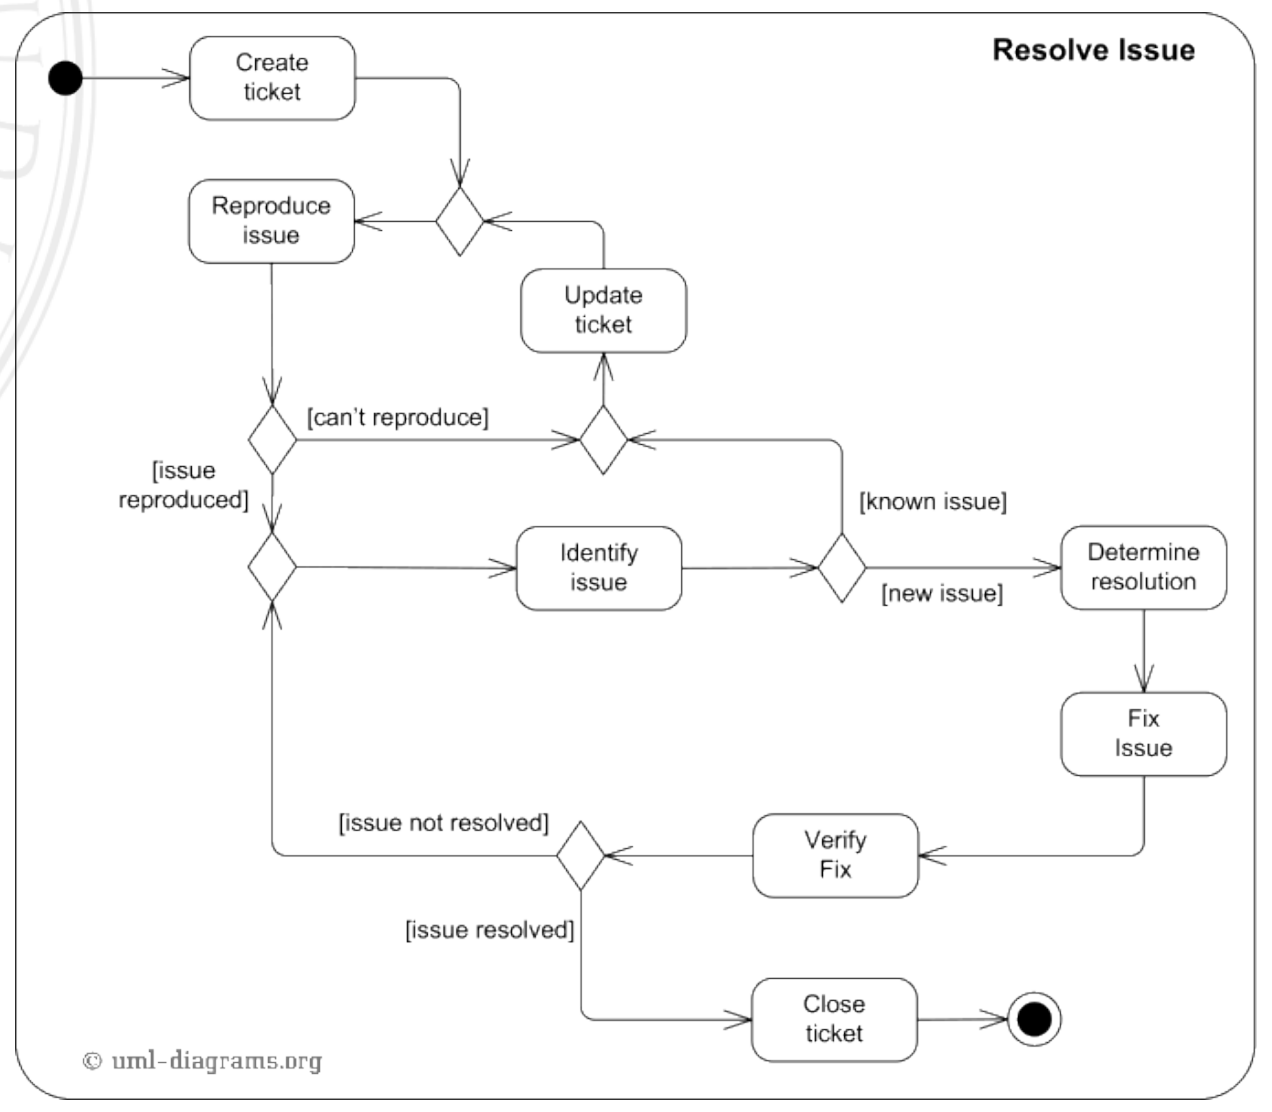
\includegraphics[width=0.8\textwidth]{foto 2.png}
\end{center}
Il pallino nero in alto a sinistra indica l'\textbf{inizio del flusso}. Il flusso ci permette di capire lo stato di avanzamento del processo stesso. Il pallino nero in basso a destra invece indica la \textbf{fine del flusso}.\\
\textit{Nota Bene}: osservando ad esempio le attività \textit{Determine resolution} e \textit{Fix issue}. La seconda potrà avvenire soltanto dopo l'esecuzione della prima.\\
Vediamo ora un altro esempio, che ci permette di osservare un'attività \textbf{parametrica}, il quale detta il funzionamento dell'attività:
\begin{center}
    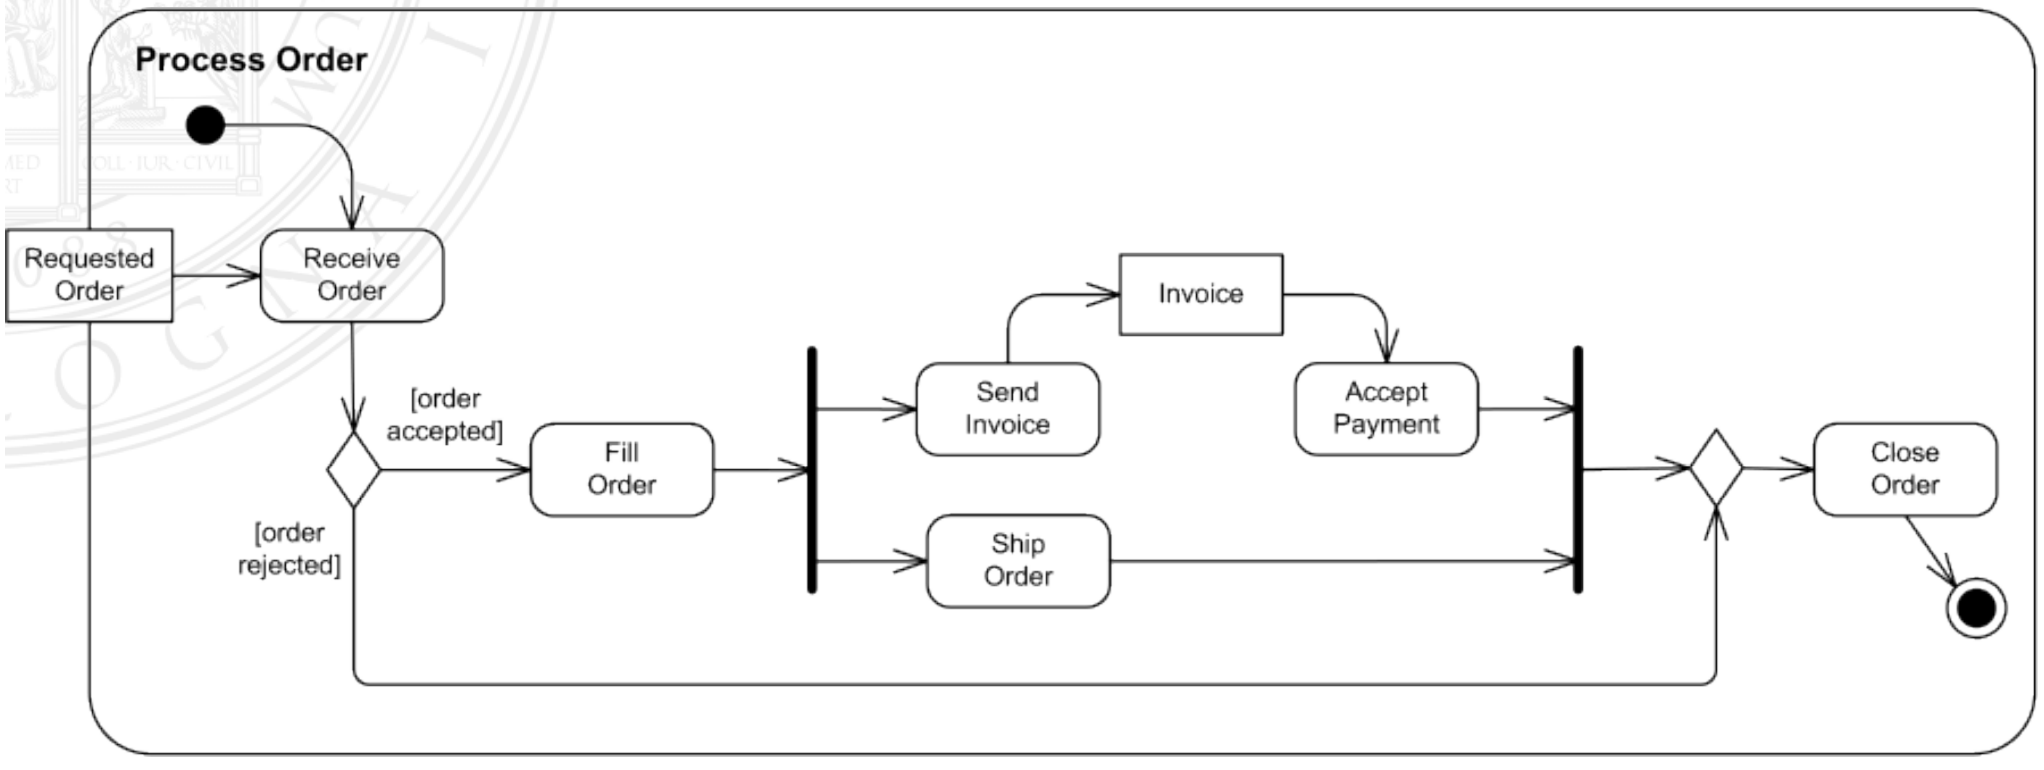
\includegraphics[width=0.8\textwidth]{foto 3.png}
\end{center}
In questo caso possiamo notare delle righe nere verticali, le quali ci indicano lo svolgimento in contemporanea di più operazioni, dividendo il flusso.\vspace{14pt}\\

\subsection*{Attività}
\large

Un'\textbf{attività} è un comportamento parametrico rappresentato come flusso coordinato di azioni. Il flusso di esecuzione è modellato come nodi di attività collegati da archi di attività.
Un'attività potrebbe essere rappresentata graficamente come un rettangolo con angoli arrotondati con il nome dell'attività nell'angolo in alto a sinistra e i nodi e gli archi dell'attività all'interno del rettangolo.
\begin{center}
    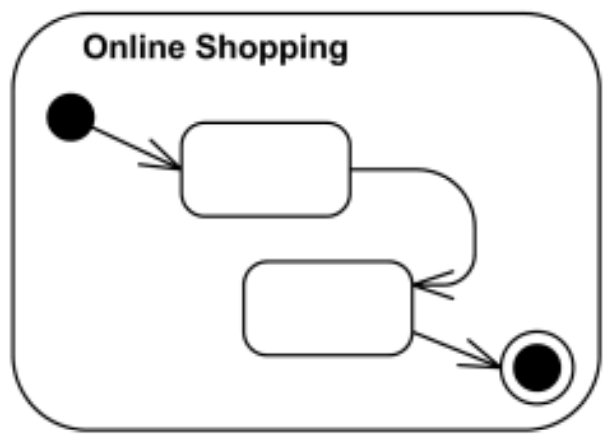
\includegraphics[width=0.3\textwidth]{foto 4.png}
\end{center}

\subsection*{Azione}
\large

Un'azione è un elemento che rappresenta un singolo passaggio atomico all’interno di un’attività. Esistono vari tipi di azioni:
\begin{enumerate}
    \renewcommand{\labelenumi}{-}
    \item occorrenze di funzioni primitive o chiamate a operazioni
    \item azioni di comunicazione, come l'invio o la ricezione di segnali
    \item manipolazioni di oggetti, come la lettura o la scrittura di attributi o associazioni
    \item invocazioni di comportamento, come attività
\end{enumerate}
Le azioni sono rappresentate graficamente come rettangoli con angoli arrotondati. Il nome o la descrizione dell'azione viene inserito all'interno del rettangolo. Un'azione può avere insiemi di archi in entrata e in uscita che specificano il flusso di controllo e flusso di dati da e verso altri nodi. Un'azione non inizierà l'esecuzione fino a quando non sarà stato completato tutto il suo input e le condizioni saranno soddisfatte.\vspace{14pt}\\
Pre-condizioni locali e post-condizioni locali sono vincoli che dovrebbero valere al momento della prima esecuzione e al suo completamento. Hanno valenza soltanto nel punto del flow che è stato specificato.
\begin{center}
    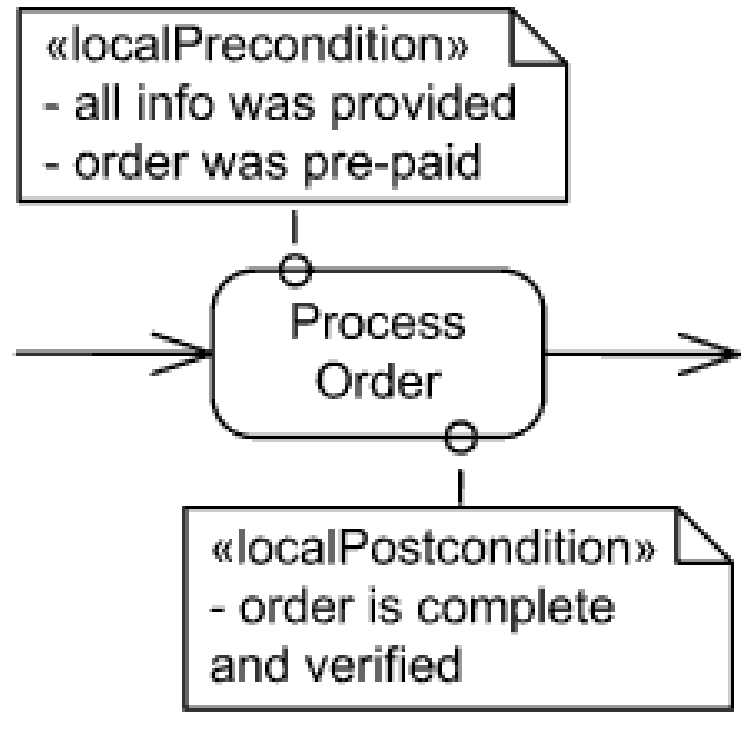
\includegraphics[width=0.35\textwidth]{foto 5.png}
\end{center}
Alcune azioni specifiche indicano degli eventi, e vengono rappresentate graficamente in maniera differente:
\begin{enumerate}
    \renewcommand{\labelenumi}{-}
    \item inviare un segnale:
    \begin{center}
        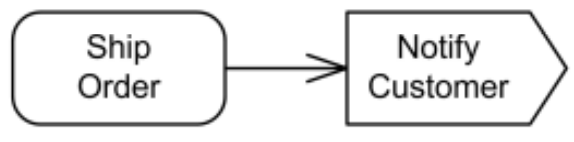
\includegraphics[width=0.3\textwidth]{foto 6.png}
    \end{center}
    \item accettare un segnale
    \begin{center}
        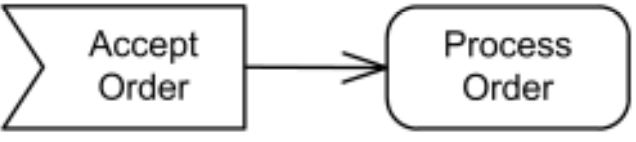
\includegraphics[width=0.3\textwidth]{foto 7.png}
    \end{center}
    \item tempo ripetuto
    \begin{center}
        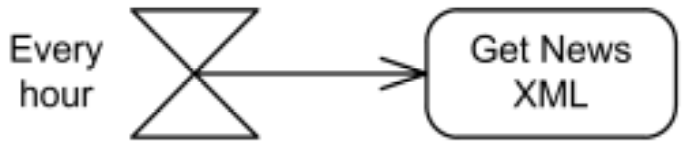
\includegraphics[width=0.3\textwidth]{foto 8.png}
    \end{center}
\end{enumerate}

\subsection*{Azione di chiamata comportamentale}
\large

Un'azione di \textbf{chiamata comportamentale} rappresenta la chiamata ad un'attività e viene indicata posizionanendo un simbolo a rastrello all'interno del simbolo dell'attività. Una notazione alternativa è di mostrare il contenuto dell'attività invocata all'interno del rentagolo arrotondato. Indica un comportamento definito da quell'azione non atomico, al suo interno le attività vengono spiegate con un altro diagramma di attività.
\begin{center}
    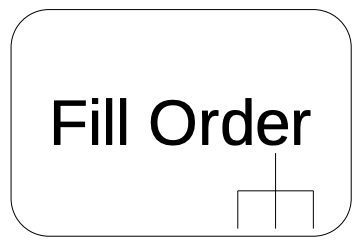
\includegraphics[width=0.25\textwidth]{foto 10.png}
\end{center}

\subsection*{Archi di attività}
\large

Un \textbf{arco di attività} è una connessione diretta tra due nodi di attività lungo i quali possono seguire il flusso i token, dal nodo dell'attività di origine al nodo dell'attività di destinazione. È una generalizzazione del flusso di controllo e degli archi del flusso degli oggetti.
Gli archi dell'attività possono avere una \textit{guardia}, specifica valutata al runtime per determinare se l'arco può essere attraversato. La \textbf{guardia} quindi valuta se il token può attraversare o meno l'arco. E' diverso dalla precondizione, nel momento che la guardia può bloccare il token.
\begin{center}
    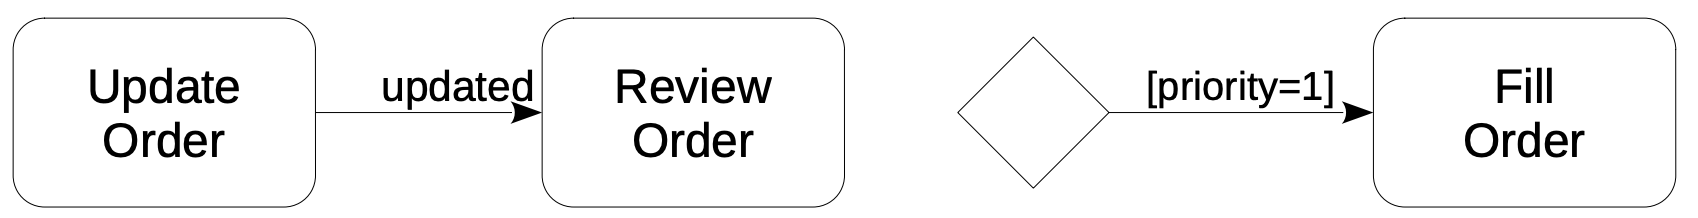
\includegraphics[width=0.8\textwidth]{foto 11.png}
\end{center}

\subsection*{Oggetto}
\large

Un \textbf{nodo oggetto} è un nodo attività di cui fa parte della definizione del flusso di oggetti in un'attività. Indica che un istanza di un particolare \textit{Classifier}, possibilmente in uno stato particolare, sia disponibile in un momento specifico dell'attività.
\begin{center}
    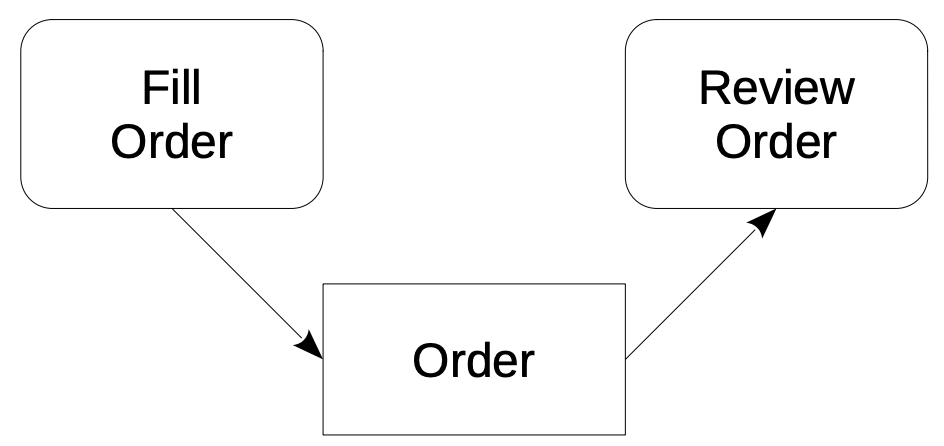
\includegraphics[width=0.5\textwidth]{foto 12.png}
\end{center}

\subsection*{Nodo di parametro di attività}
\large

ciao

\end{document}